\documentclass[11pt]{article}
\usepackage[utf8]{inputenc} % Para caracteres en espa�ol
\usepackage{amsmath,amsthm,amsfonts,amssymb,amscd}
\usepackage{multirow,booktabs}
\usepackage[table]{xcolor}
\usepackage{fullpage}
\usepackage{lastpage}
\usepackage{enumitem}
\usepackage{multicol}
\usepackage{fancyhdr}
\usepackage{mathrsfs}
\usepackage{wrapfig}
\usepackage{setspace}
\usepackage{esvect}
\usepackage{calc}
\usepackage{multicol}
\usepackage{cancel}
\usepackage{graphicx}
\graphicspath{ {pictures/} }
\usepackage[retainorgcmds]{IEEEtrantools}
\usepackage[margin=3cm]{geometry}
\usepackage{amsmath}
\newlength{\tabcont}
\setlength{\parindent}{0.0in}
\setlength{\parskip}{0.05in}
\usepackage{empheq}
\usepackage{framed}
\usepackage[most]{tcolorbox}
\usepackage{xcolor}
\colorlet{shadecolor}{orange!15}
\parindent 0in
\parskip 12pt
\geometry{margin=1in, headsep=0.25in}
\theoremstyle{definition}
\newtheorem{defn}{Definition}
\newtheorem{reg}{Rule}
\newtheorem{exer}{Exercise}
\newtheorem{note}{Note}
\newcommand{\volume}{{\ooalign{\hfil$V$\hfil\cr\kern0.08em--\hfil\cr}}}
\newcommand{\parr}{\mathbin{\|}} % Parralel Symbol
\begin{document}
\setcounter{section}{5}
\setcounter{page}{53}
\setcounter{equation}{94}

 \pagestyle{fancy}
\fancyhf{}
\rhead{Section 2: Electromagnetics}
\rfoot{Page \thepage}
\section{Amperes Law}
From Equation 80, we arrived that
\newline
\begin{equation*}
\begin{aligned}
\nabla \times \vv{H} = \vv{j}
\end{aligned}
\end{equation*}
\newline
For a current density $\vv{j}$ not due to gradient in magnetization (but rather due
to "free" current). By Stokes's theorem (Equation 73)
\newline
\begin{equation*}
\begin{aligned}
\oint_C \vv{H} \cdot \mathrm{d}\vv{l} = \int_S \vv{j} \cdot \hat{n} \, \mathrm{d}A
\end{aligned}
\end{equation*}
\newline
But this FAILS in the general case. Recall back from Equation 81 that this was the result for static cases only. Equation 81 must be modified to be completely general. In other words, we need to include the "displacement" current?

Consider a current J(t) charging a capacitor (Jahn Fig 2-3):
\begin{center}
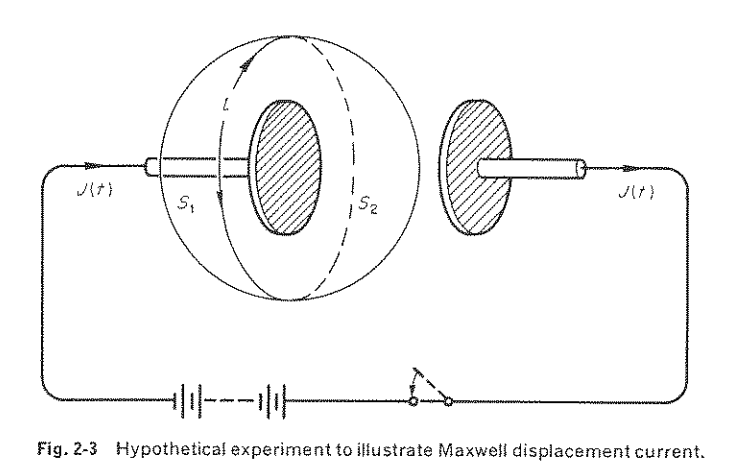
\includegraphics[scale=0.5]{4.png}
\end{center}
In this, we allow one plate of a capacitor in a simple charging circuit to be enclosed by a control surface S, around which is a closed line element $l$, which divides the surface into two sections, $S_1$ and $S_2$. $S_1$ is the input end while $S_2$ is the output end of the electrode. When the switch is closed, a current J(t) flows around the circuit to charge the two capacitor plates.
\newpage
Applying the previously-derived version of Ampere's law (Equation 80 and Equation 81) to contour C and surface $S_1$ we get:
\newline
\begin{equation*}
\begin{aligned}
\oint_C \vv{H} \cdot \mathrm{d}\vv{l} = \int_{S_1} \vv{j} \cdot \hat{n} \, \mathrm{d}A = J(t)
\end{aligned}
\end{equation*}
\newline
But $l$ is also  a boundary for $S_2$, and no current flows through that surface. Hence, we should infer the contradiction:
\newline
\begin{equation*}
\begin{aligned}
\oint_C \vv{H} \cdot \mathrm{d}\vv{l} = \int_{S_2} \vv{j} \cdot \hat{n} \, \mathrm{d}A = 0
\end{aligned}
\end{equation*}
Clearly this needs modification for transient situations since
\newline
\begin{equation*}
\begin{aligned}
\int_{S_2} \vv{j} \cdot \hat{n} \, \mathrm{d}A -  \int_{S_1} \vv{j} \cdot \hat{n} \, \mathrm{d}A \neq 0
\end{aligned}
\end{equation*}
\newline
The result of which means that in order to sum to 0, $\frac{\partial \rho}{\partial t} = 0$ which is not ideal. The reason why requires us to consider current continuity:
\newline
\begin{equation*}
\begin{aligned}
\frac{\partial \rho_e}{\partial t} + \nabla \cdot \vv{j} = 0
\end{aligned}
\end{equation*}
If
\begin{equation*}
\begin{aligned}
\frac{\partial \rho_e}{\partial t} = 0 \quad \text{(Static)} \rightarrow \nabla \cdot \vv{j} = 0 
\end{aligned}
\end{equation*}
\newline
But we are missing a time-varying $\rho_e$

The net charge within the control volume is changing with time and therefore is NOT equal to zero because charge is accumulating on the capacitor plate. The capacitor is being charged.

Now we see why Equation 80, $\nabla \times \vv{H} = \vv{j}$, is inadequate, it doesn't
satisfy current continuity.

We can fix discrepancy by adding a term. Since (Equation 35)
\newline
\begin{equation*}
\begin{aligned}
\nabla \cdot \vv{D} = \rho_e
\end{aligned}
\end{equation*}
Then
\begin{equation*}
\begin{aligned}
\frac{\partial}{\partial t}  \nabla \cdot \vv{D} = \frac{\partial \rho_e}{\partial t} 
\end{aligned}
\end{equation*}
\newline
Now, we can write current continuity (Equation 55) as
\newline
\begin{equation*}
\begin{aligned}
\frac{\partial}{\partial t}(\nabla \cdot \vv{D}) + \nabla \cdot \vv{j} = 0
\end{aligned}
\end{equation*}
Or
\begin{equation}
\begin{aligned}
\nabla \cdot (\vv{j} + \frac{\partial \vv{D}}{\partial t}) = 0
\end{aligned}
\end{equation}
\newpage
The correct form of the magnetic intensity ("H"-Field) equation then
becomes the:
\begin{shaded}
\textbf{Generalized Form of Ampere's Law}
\begin{equation}
\begin{aligned}
\nabla \times \vv{H} = \vv{j} + \frac{\partial \vv{D}}{\partial t}
\end{aligned}
\end{equation}
Where
\begin{equation*}
\begin{aligned}
\frac{\partial \vv{D}}{\partial t} &= \text{Displacement Current} \\ \\
\vv{j} + \frac{\partial \vv{D}}{\partial t} &= \text{Generalized Current Density}
\end{aligned}
\end{equation*}

Previously we assumed (in Equation 81) that fields were independent of time or
slowly varying, so $\frac{\partial \vv{D}}{\partial t} < < \vv{j}$ for Equation 80 and Equation 81.
\end{shaded}

To summarize and tie things back to Fig. 2-3 above, Maxwell resolved this inconsistency by arguing that in the process of charging the capacitor in this way, an electric field is caused to increase between the plates and that this time rate of change of $\vv{E}$ is equivalent to a real current density for the purposes of induction of an "H"-field. However, to be dimensionally consistent, it is the time derivative of $\vv{D}$, the source field, not $\vv{E}$, that is needed.
\newpage
\section{Maxwell's Equations - Summary}
We now have all the background information required to write Maxwell's Equations:
\newline
\begin{equation*}
\begin{aligned}
\nabla \times \vv{H} &= \vv{j} + \frac{\partial \vv{D}}{\partial t} &\qquad &\textbf{Loi d'Amp\`{e}re}\\ 
&&&\text{The curl of the H-field is due to a time-varying displacement current} \\
&&&\text{and the applied current.}\\
&&&\text{\emph{\underline{Meaning:}}}\\
&&&\text{The magnetic field induced around a closed loop is proportional to}\\
&&&\text{the electric current plus displacement current (rate of change of }\\
&&&\text{electric field) that the loop encloses.}
\\ \\
\nabla \times \vv{E} &= \frac{\partial \vv{B}}{\partial t} &\qquad &\textbf{Loi de Faraday}\\
&&&\text{The curl of the E-field is due to a time-varying B-field}\\
&&&\text{\emph{\underline{Meaning:}}}\\
&&&\text{The voltage induced in a closed loop is proportional to the rate}\\
&&&\text{of change of the magnetic flux that the loop encloses.}
\\ \\
\nabla \cdot \vv{D} &= \rho_f & \qquad &\textbf{Loi de Gauss}\\
&&&\text{The divergence of the displacement current is due to the free charge} \\
&&&\text{\emph{\underline{Meaning:}}}\\
&&&\text{The electric flux leaving a volume is proportional to the charge inside.}
\\ \\
\nabla \cdot \vv{B} &= 0 & \qquad &\textbf{Loi Monopole} \\
&&&\text{The divergence of the B-field is 0}\\
&&&\text{\emph{\underline{Meaning:}}}\\
&&&\text{Magnetic Monopoles do not exist; the total magnetic} \\
&&&\text{flux through a closed surface is zero.}
\end{aligned}
\end{equation*}
\newline
When dealing with material bodies, we need constitutive relations, meaning we need to know how those materials respond to Electric and Magnetic fields:
\newline
\begin{equation*}
\begin{aligned}
\vv{D} &= \epsilon(\vv{E}) \, \vv{E} &\qquad \qquad& \text{Equation 39} \\ \\
\vv{H} &= \mu(\vv{B}) \, \vv{B} &\qquad \qquad& \text{Equation 83}
\end{aligned}
\end{equation*}
\newline
Finally, we need a force equation to model the forces on charged particles, Lorentz Force Equation (Equation 66):
\begin{equation*}
\begin{aligned}
\vv{F} = q \, (\vv{E} + \vv{v} \times \vv{B})
\end{aligned}
\end{equation*}
\newpage
\end{document}